\section{The hourly forward curve}
\label{sec:curve}

Figure~\ref{fig:pipeline} summarises how the components of the framework fit
together and, more importantly, where market information enters and where it
does not. The upper path carries observed prices into the forward curve. The
lower path carries historical estimates into the residual dynamics. The two
meet only at the centring step, and the separation is what makes the
identification argument of this paper possible.

\begin{figure}[htbp]
\centering
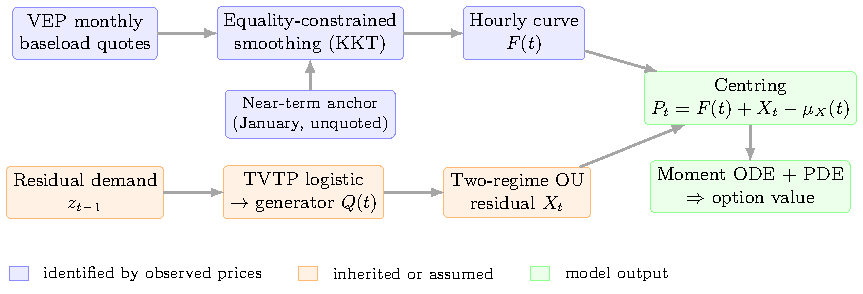
\includegraphics[width=0.92\textwidth]{figures/pipeline.pdf}
\caption{Structure of the valuation framework. Blue elements are identified by
observed prices; orange elements are inherited from historical estimation or
assumed. Only the first moment of the price distribution is determined by the
market path; volatility and regime risk premia are not. (Vector source:
\texttt{figures/pipeline\_src.tex}.)}
\label{fig:pipeline}
\end{figure}

\subsection{The averaging constraint}

Let $\mathcal{H}_m$ denote the set of delivery hours of month $m$ and
$\mathrm{VEP}_m$ the observed baseload quote. Settlement against the arithmetic
mean imposes
\begin{equation}
  \frac{1}{|\mathcal{H}_m|}\sum_{h\in\mathcal{H}_m} F(h) \;=\; \mathrm{VEP}_m,
  \qquad m \in \mathcal{M},
  \label{eq:monthly}
\end{equation}
where $\mathcal{M}$ is the set of quoted months. With $N$ hourly unknowns and
$|\mathcal{M}|=6$ constraints, the system is massively underdetermined: in our
configuration $N=5{,}089$ and the constraints fix six linear functionals. The
remaining $N-6$ degrees of freedom are chosen, not identified. We select them by
a smoothness criterion, and we regard that selection as an assumption on the
same footing as any other, not as an estimation result.

\subsection{Roughness-penalised construction}

Write $\mathbf{F}\in\mathbb{R}^{N}$ for the vector of hourly forward prices and
$D_2\in\mathbb{R}^{(N-2)\times N}$ for the second-difference operator,
$(D_2\mathbf{F})_i = F_{i+2}-2F_{i+1}+F_i$. Let $\mathbf{B}$ be a piecewise
baseline that is constant at $\mathrm{VEP}_m$ within each quoted month and
follows the near-term anchor rule of Section~\ref{sec:anchor} elsewhere. The
curve solves
\begin{equation}
  \min_{\mathbf{F}} \;
    w_R\,\lVert D_2\mathbf{F}\rVert_2^{2}
    \;+\; w_A\,\lVert \mathbf{F}-\mathbf{B}\rVert_2^{2}
  \quad\text{subject to}\quad
  A\mathbf{F}=\mathbf{b},
  \label{eq:qp}
\end{equation}
where each row of $A$ implements one instance of \eqref{eq:monthly}, together
with the anchor row. This is a convex quadratic program with linear equality
constraints, and we solve it as a single sparse Karush--Kuhn--Tucker system,
\begin{equation}
  \begin{bmatrix}
    2\left(w_R D_2^{\top}D_2 + w_A I\right) & A^{\top}\\
    A & 0
  \end{bmatrix}
  \begin{bmatrix}\mathbf{F}\\ \boldsymbol{\lambda}\end{bmatrix}
  =
  \begin{bmatrix}2w_A\mathbf{B}\\ \mathbf{b}\end{bmatrix}.
  \label{eq:kkt}
\end{equation}

Because the quotes enter as equality constraints rather than as penalty terms,
the weights $w_R$ and $w_A$ govern only the shape of the curve within months.
They cannot trade off fit against smoothness, and no choice of weights can
violate \eqref{eq:monthly}. This has a consequence for how the resulting fit
should be read, and we state it plainly because the opposite reading is the
natural one: the monthly reproduction error we report in
Section~\ref{sec:curvefit} is of order $10^{-12}$ \TRY, and that number is a
property of the solver, not evidence about the model. A formulation that
reproduces its inputs by construction has not been tested by reproducing them.

\subsection{The unquoted near-term window}
\label{sec:anchor}

January 2026 has no quote, and every option maturity examined here falls inside
it. This is not a gap peculiar to one date. Across the seven valuation dates
used in Section~\ref{sec:multidate}, spanning December 2022 to December 2025,
the nearest delivery month is unquoted at every one: the front contract is
delisted before the month it delivers into begins, so a participant valuing a
short-dated instrument never observes a forward price for the period that
instrument covers. The level over that window must therefore come from an
assumption, and the assumption is a permanent feature of valuation in this
market rather than an occasional inconvenience. Three rules are considered, all
respecting the observed spot at the valuation hour where applicable:

\begin{enumerate}
\item \textbf{\texttt{spot\_flat}}: hold the observed spot $2{,}917.78$ \TRY{}
      flat across the window;
\item \textbf{\texttt{spot\_to\_next\_linear}}: interpolate linearly from the
      observed spot at $t_0$ to the February quote at the month boundary;
\item \textbf{\texttt{flat\_next\_month}}: hold the February quote flat
      backwards across January.
\end{enumerate}

We adopt \texttt{spot\_to\_next\_linear} as the production rule on three
grounds. It satisfies $F(t_0)=P_{t_0}$, so the curve is consistent with the one
spot observation that is not in dispute. It joins the February quote without a
discontinuity at the month boundary, with a residual jump of $0.05$ \TRY{}
against $12$--$47$ \TRY{} at boundaries elsewhere in the curve. And it produces
a non-degenerate term structure across the window, whereas
\texttt{flat\_next\_month} violates $\E[P_{t_0}]=P_{t_0}$ by $17$ \TRY{} and
\texttt{spot\_flat} embeds an unmotivated claim that January is a high-price
month relative to February. Section~\ref{sec:anchorsens} quantifies how much
this choice moves option values, which is the question that matters more than
the choice itself.

\begin{remark}
The near-term anchor is the weakest link in the market path of
Figure~\ref{fig:pipeline}, and its weakness is structural rather than
remediable within the data. Where no quote exists for the delivery period, no
construction can identify its forward level; it can only be assumed, and the
assumption should be reported as a sensitivity range rather than a point.
\end{remark}
